\chapter{Evaluation}\label{ch04_evaluation}

In this section, we will analyze and evaluate the results of our methods, considering their quality and effectiveness. To provide a comprehensive understanding, 
we will present various plots and visualizations to support our findings and observations. These plots will serve as quantitative and visual evidence of the outcomes achieved through our approach. 

\section{Reconstruction Accuracy}\label{sec:reconstruction_accuracy}

Our initial experiment aims to assess the reconstruction accuracy achieved through the application of Principal Component Analysis (PCA). 
To conduct this experiment, we compare the reconstructed 3D models generated using varying numbers of principal components to the original input models. 
We calculate and analyze the reconstruction error, which quantifies the dissimilarity between the original models and their reconstructions.

\begin{figure}[H]
    \centering
    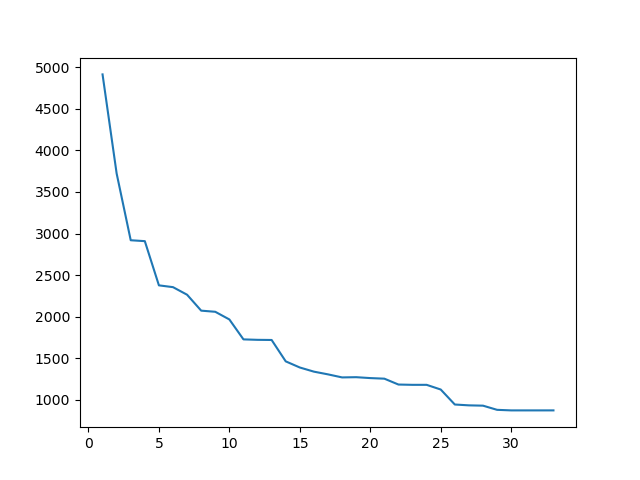
\includegraphics[width = 0.8\textwidth]{figures/plot_recreation_accuracy.png}
    \caption{Reconstruction Accuracy}
    \label{fig:reconstruction_accuracy}
\end{figure}

Figure \ref{fig:reconstruction_accuracy} shows hat we can clearly see the first few principal components are the most important ones. It is important to note that the method of calculating the dissimilarity is done by summing up
the euclidean distances between the vertices of the original and reconstructed models:
\[\sum \lVert v_i - u_i \rVert\]
where $v_i$ is the $i$th vertex of the original model and $u_i$ is the $i$th vertex of the reconstructed model. Given the non-normalized nature of the vertex coordinates, 
we interpret this distance as a form of relative distance rather than an absolute measurement. Yet figure \ref{fig:reconstruction_accuracy} still shows relevant information.


\section{Correction UI}

\subsection{L-BFGS-B}

Here we discuss the implementation of SciPy's L-BFGS-B minimization algorithm. SciPy's implementation of scipy.minimize() allows to choose many minimization algorithms. Because we have a parallel implementation of the 
L-BFGS-B algorithm, we compare it to the serial implementation of the L-BFGS-B algorithm. 

The principal parameters in which we are interested in are the number of iteration and the number of principal components changed. We will show the effect of these parameters on the execution time and the loss.

\begin{figure}
    \centering
    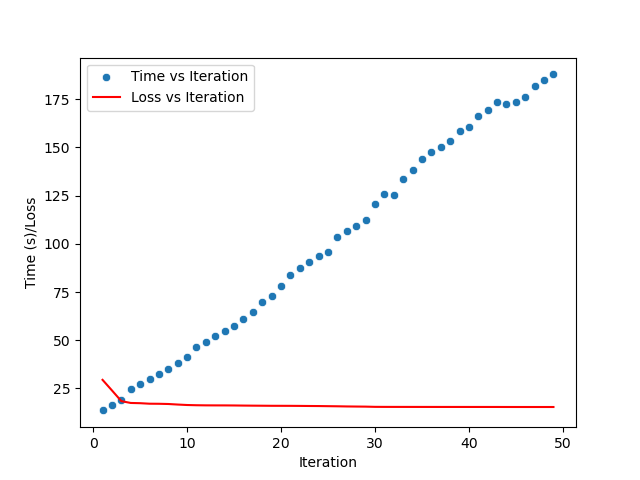
\includegraphics[width = 0.8\textwidth]{figures/plot_quasiNewton_serial.png}
    \caption[Serial quasi Newton: time and loss vs iterations]{Plot of the serial quasi Newton method showing execution time and loss vs the number of iterations}
    \label{fig:plot_quasiNewton_ser_time}
\end{figure}

\begin{figure}[H]
    \centering
    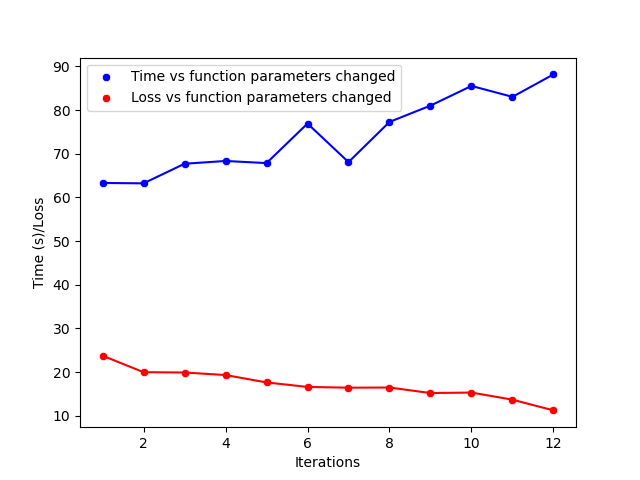
\includegraphics[width = 0.8\textwidth]{figures/plot_quasiNewton_ser_fun_params.png}
    \caption[Serial quasi Newton: time and loss vs principal components]{Plot of the serial quasi Newton method showing execution time and loss vs the number of principal components changed}
    \label{fig:plot_quasiNewton_ser_fun_params}
\end{figure}

Figure \ref{fig:plot_quasiNewton_ser_time} shows the execution time and loss of the serial Quasi Newton method vs the number of iterations. We see a linear increase in the execution time, while after a certain
number of iterations the loss does only decrease slightly. This means that if we wanted to implement this method, we would have to stop the optimization after a few number of iterations.

Figure \ref{fig:plot_quasiNewton_ser_fun_params} shows the execution time and loss of the serial Quasi Newton method vs the number of principal components changed. We kept the number of iterations constant to 10, in contrast to
the findings in figure \ref{fig:plot_quasiNewton_fun_params}, so we can not directly compare the results. We interpret increase in execution time as linear, while we interpret the decrease in loss also as linear. This is in contrast
to the parallel implementation, which we discuss later.

\subsection{Parallel L-BFGS-B}

In this part we analyze the results of our implementation and experimentation with the parallel L-BFGS-B algorithm. As discussed in \ref{sec:lbfgsb},
we have multiple options in implementing this method. We show the effect of a number of changes in the implementation of the algorithm.

\begin{figure}[H]
    \centering
    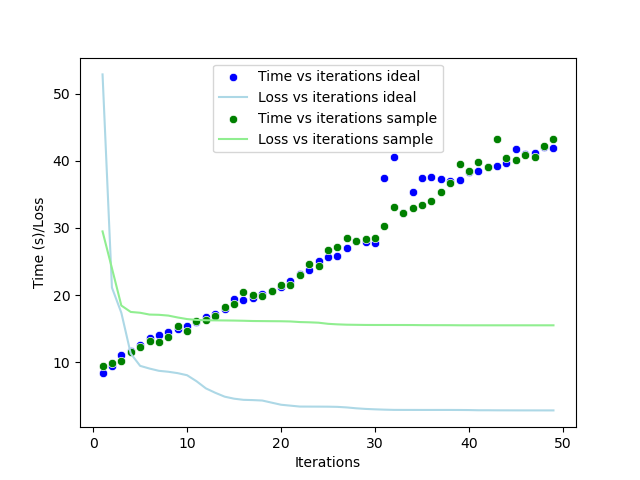
\includegraphics[width = 0.8\textwidth]{figures/plot_quasiNewton_time.png}
    \caption[Parallel quasi Newton: time and loss vs iterations]{Plot of the parallel Quasi Newton method showing execution time and loss vs the number of iterations}
    \label{fig:plot_quasiNewton_time}
\end{figure}

\begin{figure}[H]
    \centering
    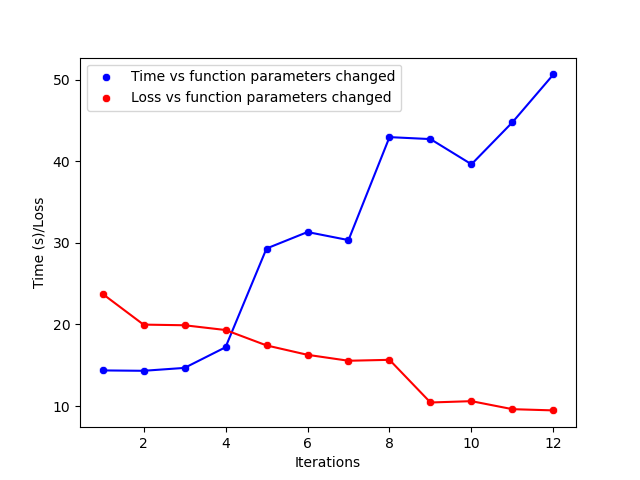
\includegraphics[width = 0.8\textwidth]{figures/plot_quasiNewton_fun_params.png}
    \caption[Parallel quasi Newton: time and loss vs principal components]{Plot of the Quasi Newton method showing execution time and loss vs the number of principal components changed}
    \label{fig:plot_quasiNewton_fun_params}
\end{figure}

\begin{figure}[H]
    \centering
    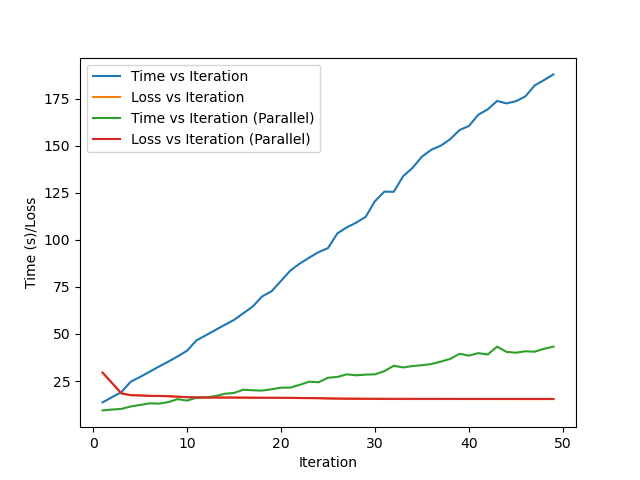
\includegraphics[width = 0.8\textwidth]{figures/plot_quasiNewton_serial_vs_parallel.png}
    \caption[Parallel vs sequential quasi Newton]{Plot of the Quasi Newton method showing execution time and loss vs the number of principal components changed in the serial and parallel implementation}
    \label{fig:plot_quasiNewton_time_ser_vs_par}
\end{figure}

Figure \ref{fig:plot_quasiNewton_time} shows the execution time and loss of the parallel Quasi Newton method vs the number of iterations. We also have two models and corresponding objective lines to
show the difference between a real world application, meaning a user drawn line, and a line which is a perfect fit to the model. \ref{fig:ui_correction} shows the exact model and line we used for our measurements. We see a very steep drop in the loss in the first few iterations,
which is to be expected. This means that if we had used this implementation we would have been able to achieve a very reasonable result with just a few iterations.

Figure \ref{fig:plot_quasiNewton_fun_params} shows the execution time and loss of the parallel Quasi Newton method vs the number of principal components changed. We kept the number of iterations constant to 30
As expected, the execution time goes up, the more principal components we change. This is because the number of parameters we have to optimize increases, 
and thus the number of function evaluations increases. The loss also decreases as we increase the number of principal components changed, which is to be expected.

In contrast to \ref{fig:plot_quasiNewton_ser_fun_params}, the way how the execution time increases is not as clear to see. But what we can see is that we hit a plateau when we change seven parameters. As discussed in \ref{sec:lbfgsb},
this is expected. If we wanted to implement our correction UI with the parallel L-BFGS-B algorithm, we would choose to change seven parameters.

Figure \ref{fig:plot_quasiNewton_time_ser_vs_par} shows the execution time and loss of the parallel and serial Quasi Newton method vs the number of iterations in the parallel and the serial implementation. 
We can clearly notice, that the difference between the losses is very small, while the difference in execution time is very large. This is not very surprising, as we expect a constant speedup, as mentioned in \ref{sec:lbfgsb}.

\subsection{Newton's Method}

Now we discuss our actual implementation, which uses Newton's method. We primarily focus on the number of iterations in conjunction with the loss, meaning the function to minimize. For an explanation of our implementation refer to
\ref{sec:methods} and \ref{sec:implementation}. We note here that the execution time of our Newton method is very small compared to the execution time of the parallel L-BFGS-B algorithm.

\begin{figure}[H]
    \centering
    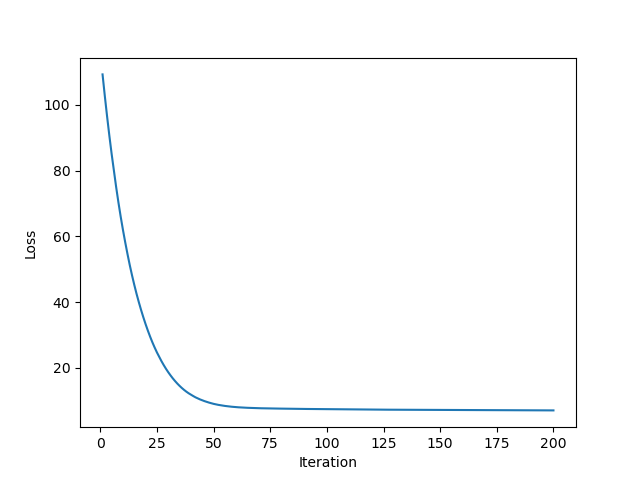
\includegraphics[width = 0.8\textwidth]{figures/plot_losses.png}
    \caption[Newton's method: loss vs iteration]{Plot showing losses vs iterations}
    \label{fig:losses_vs_iterations}
\end{figure}

\begin{figure}[H]
    \centering
    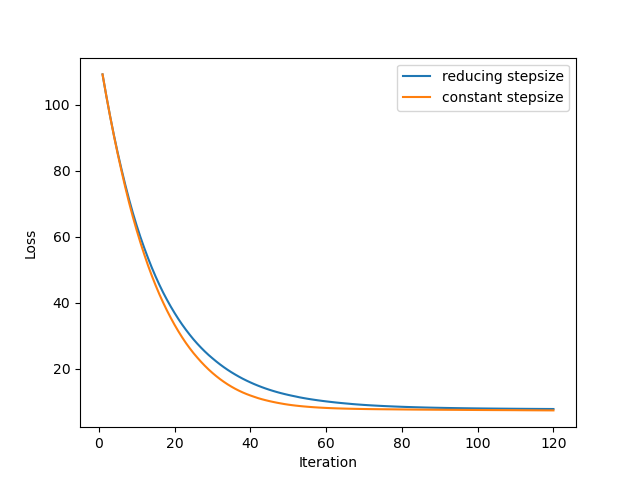
\includegraphics[width = 0.8\textwidth]{figures/plot_losses_vs_iterations_stepsize.png}
    \caption[Newton's method: reducing step size]{Plot showing losses vs iterations with and without a reduction of the step size}
    \label{fig:losses_vs_iterations_stepsize}
\end{figure}

Figure \ref{fig:losses_vs_iterations} shows the loss vs the number of iterations of our implementation of Newton's method. We see the loss decreasing very quickly in the first few iterations. It is important
to note that here a single iteration only takes a few milliseconds, so here 200 iterations are a lot quicker than 50 iterations of the parallel L-BFGS-B algorithm. In our implementation we chose to stop the optimization
after 100 iterations.

In figure \ref{fig:losses_vs_iterations_stepsize} we show the loss vs the number of iterations with and without a reduction of the step size. Here the step size is multiplied by $0.99$ after every iteration, and starts with one, 
meaning in the first iteration we go in the negative direction of the gradient equal to the gradient. We observe that the loss decreases slower than without the reduction of the step size, but after 90 iterations we have more
or less the same loss again. This is why we didn't use a reduction of the step size in our implementation.

\subsubsection{Execution Time of our Implementation}
As described in \ref{sec:implementation} the execution time does not depend on the number of parameters we change, but only on the number of iterations, and the time it takes to calculate the minimal difference between the
breast and the line. Since the number of iterations is constant, we only have to look at the time it takes to calculate the difference. Here the more point the line has, meaning the more point the line has, the longer it takes to calculate the difference.

In figure \ref{fig:plotlenline} one can see the execution time vs the length of the list. Here we clearly see a linear behavior. What also can be seen is that the execution time is very small as displayed in Table \ref{tab:time_table}.

\begin{figure}[H]
    \centering
    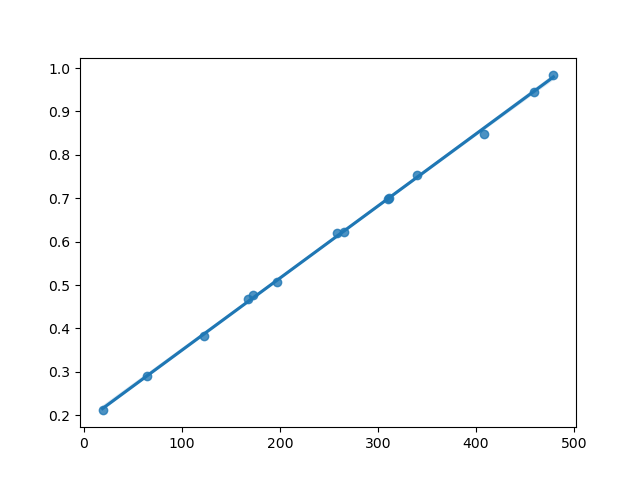
\includegraphics[width = 0.8\textwidth]{figures/plot_newtonMethod_line_len.png}
    \caption[Newton's method: execution time vs length of line]{Plot showing the execution time vs the length of the line}
    \label{fig:plotlenline}
\end{figure}

\begin{table}
    \centering
    \begin{tabular}{||c c||}
        \hline
        Length of the line & Execution time in seconds\\ \hline \hline
        19 & 0.211901\\ \hline
        64 & 0.29\\ \hline
        123 & 0.3821\\ \hline
        167 & 0.4668\\ \hline
        172 & 0.4764\\ \hline
        197 & 0.507099\\ \hline
        258 & 0.6202\\ \hline
        265 & 0.623\\ \hline
        310 & 0.6987\\ \hline
        311 & 0.7006\\ \hline
        340 & 0.7527\\ \hline
        408 & 0.8482\\ \hline
        459 & 0.9456\\ \hline
        479 & 0.9836\\\hline
    \end{tabular}
    \caption[Execution time and length of line]{Execution time of our implementation of Newton's method and the length of the line}\label{tab:time_table}
\end{table}
